\documentclass[main]{subfiles}
\begin{document}

%@@@@@@@@@@@@@@@@@@@@@@@@@@@@@@
% Main Topics: Synapse I 01.11.2018
% Lecturer: Daniel Kiper
% author: Vanessa Leite - base document from benelot/eth-intro-to-neuroinformatics-summary

\section{Synapse}
\subsection{Introduction}
\begin{itemize}[noitemsep,nolistsep]
	\item First mentioned by Sherrington (1873).
	\item Cajal's golgi staining methods suggested the presence of contacts between cells that were used for communication ~1900's.
	\item Otto Loewi experimented with the vagus nerve~\ref{fig:vagus-experiment}.
	\subitem Stimulating the vagus nerve slows down the heart beat, has an inhibitory function.
	\subitem Ringers solution is a mixture of chemicals in which the heart can continue beating.
	\subitem When switching the solution with one that has been used with an activated vagus nerve, the heart will slow down.
	\item It was found that the ``Vagusstoff'' is acetylcholine (ACh).
	\item The synapses are receptive for nicotine, muscarine and acetylcholine, because of ACh-receptors. This makes certain substances very addictive.
	\item Residual acetylcholine has to be cleared and removed immediately. This happens with acetylcholine esterase enzymes.
\end{itemize}

\begin{figure}[H]
	\centering
 	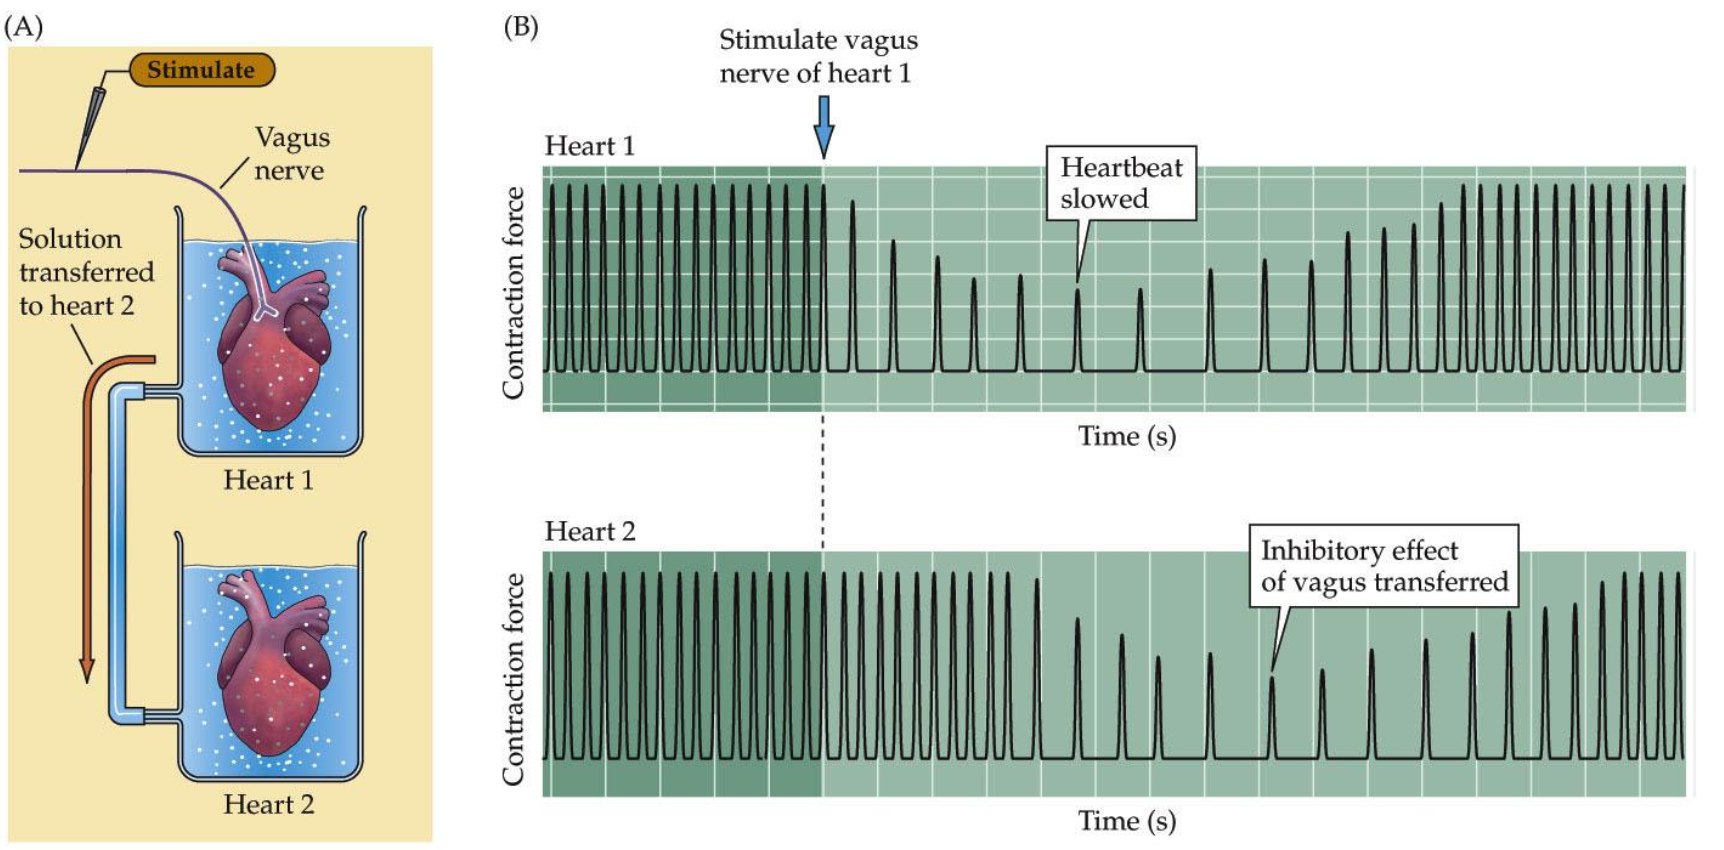
\includegraphics[width=0.8\textwidth]{vagus-nerve-experiment.png}
 	\caption{Otto Loewi vagus experiment. Two solutions connected, one heart in each. After stimulation of one of them, the other one, after a short time, has the same effect.}
 	\label{fig:vagus-experiment}
\end{figure} 

\subsubsection{Soup vs Spark - Chemical or Electrical?}
Evidence for chemical transmission at the neuro muscular junction was widely accepted by neuropharmacologists. However, some physiologists thought that certain aspects were too fast to be mediated chemically.
Chemical synapses is the predominant way of communication between neurons, but there are some electrical synapses.

\subsection{Chemical transmission}
Communication between cells which involves the rapid release and diffusion of a substance to another cell where it binds to a receptor (at a localized site) resulting in a change in the postsynaptic cells properties.

\begin{itemize}
\item synaptic cleft: $20$ to $40nm$.
\item vesicles in presynaptic terminal
\item neurotransmitters ($>1000$ per vesicle)
\item neurotransmitters released by depolarization, $Ca^{2+}$ dependent
\item vesicles are released by exocytose in the active zone (specialized site in presynaptic neuron for release).
\item diffusion
\item binding to receptors
\item channel opening
\item amplification
\item Multiple steps are required to release transmitter chemicals and for them to act on postsynaptic receptors, resulting in a time delay (can be as short as $0.2 ms$, from $Ca^{2+}$ entry to secretion).
\item Directional, select localization of release machinery to presynaptic terminals and receptors to postsynaptic specializations. 
\item Can change sign by release of inhibitory transmitter.
\end{itemize}

\subsubsection{Steps of transmission}
\begin{itemize}
\item Action potential generated and reach the axon of presynaptic cell
\item Opening of voltage gate $Ca^{2+}$ channels
\item Diffusion and action of $Ca^{2+}$ at release machinery
\item Exocitosys and diffusion of transmitter in cleft
\item Activation of post-synaptic cell
\end{itemize}

\paragraph{Model of synaptic transmission}
Neurotransmitter is released in discrete packages, or quanta.
Quantal size: size of individual quanta.
Quantal content: number of quanta released.

\begin{itemize}
\item One package of neurotransmitter = one quantum
\item AP transiently increases the probability of releasing NX quanta.
\item Several quanta are available to be released
\item Each quantum give approximately the same postsynaptic response: quantal amplitude.
\item the average number of quanta released: $m = np$
\subitem $n$ is the number of quanta available for release
\subitem $p$ their average release probability 
\item Probability that $x$ units successfully contribute is given by: $P(success = x) = \binom{n}{x} p^x (1-p)^x$
\end{itemize}

\subsubsection{Synapse properties}
\begin{itemize}[noitemsep,nolistsep]
	\item Only vesicles which are already on the presynaptic membrane (docked) will be released after the AP, not all of them.
	\item One single synapse produces only a small potential. More are needed for an actual action potential.
	\item Release of neurotransmitters is calcium dependent.
	\item Probabilistic release of neurotransmitter.
	\subitem In the CNS, most of the time only one vesicle is released with probability $0.2$ to $0.4$.
	\subitem An amplitude histogram shows poisson distribution, which gives the probability of firing.
	\subitem The action potential (probability of firing of synapses, probability of postsynaptic receptors to bind neurotransmitter) give the plasticity (overall probability of passing action potential to postsynaptic neuritic changes).
	\item Single activated synapse is usually not enough. EPSP is about $0.1\,mV$.
	\item The current-voltage lines have bio-measured sigmoid-curves, because channels open with a probability.
	\item Four types of synapse: axodendritic, axosomatic, axoaxonic and dendrodendritic.
\end{itemize}

\subsubsection{Synaptic mechanism}

\begin{enumerate}[noitemsep,nolistsep]
	\item Synthesis: Building blocks of transmitter substance gets to the terminal where neurotransmitter is synthesized and packed into vesicles.
	\item Release: In response to an AP, the transmitter is released, across the membrane, by exocytosis. The presynapse has voltage-gated $Ca^{2+}$ channels, which will cause an inflow and trigger vesicle fusion (exocytosis).
	\item Receptor activation: The transmitter crosses the synaptic cleft and binds to a receptor.
	\item Inactivation: The transmitter is taken back or inactivated in the synaptic cleft.
\end{enumerate}


\subsubsection{Receptor types}
Neurotransmitters cross synaptic-cleft and can bind to two types of receptors: ionotropic (ligand-gated ion channels) or metabotropic (g-protein coupled receptors).

\begin{tabular}{|l|l|}
	\hline
	\textbf{Ionotropic receptor} & \textbf{Metabotropic receptor}\\\hline
	Binding site + channel combined & Binding site not associated with channel\\\hline
	Second messenger independent & G-protein or second messenger involved\\\hline
	Short latency action & Longer latency\\\hline
	Rapid response (10 to 50 ms) & Slow responses\\\hline
	Postsynaptic, in general & Pre- and postsynaptic\\\hline
\end{tabular}

\subsubsection{Synapse types}
\begin{tabular}{|l|l|}
	\hline
	\textbf{Electrical synapse} & \textbf{Chemical synapse}\\\hline
	Simple primitive system & Highly developed structure\\\hline
	Often symmetrical, bidirectional & Polarized, structurally and functionally\\\hline
	Gap junction (connexins) & Pre: active zone, post: postsynaptic density\\\hline
	Very fast, no synaptic delay & Slower, synaptic delay (0.5 ms)\\\hline
	$Ca^{2+}$-independent & Transmitter release requires $Ca^{2+}$ influx\\\hline
	Large synapse & Thousands of small synapses\\\hline
	Limited functions, usually excitatory & Versatile: Excitatory and inhibitory\\\hline
	Synchronized activity & Specific: point to point communication\\\hline
\end{tabular}

\subsubsection{Receptor overview}
\begin{tabular}{|l|l|l|l|l|}
	\hline
	\textbf{Receptor} & \textbf{Transmitter} & \textbf{Ions} & \textbf{Approx. $E_{rev}$} & \textbf{Agonist}\\\hline
	AMPA & glutamate & Na, K, Ca & $+0\,mV$ & AMPA\\\hline
	NMDA & glutamate & Na, K, Ca & $+0\,mV$ & NDMA\\\hline
	mGLU & glutamate & G-coupled & & \\\hline
	$GABA_A$ & gaba & Cl & $-65\,mV$ & muscimol\\\hline
	$GABA_B$ & gaba & K & $-90\,mV$ & \\\hline
\end{tabular}

\begin{figure}[H]
	\centering
	\begin{subfigure}[b]{0.5\textwidth}
    	\centering
		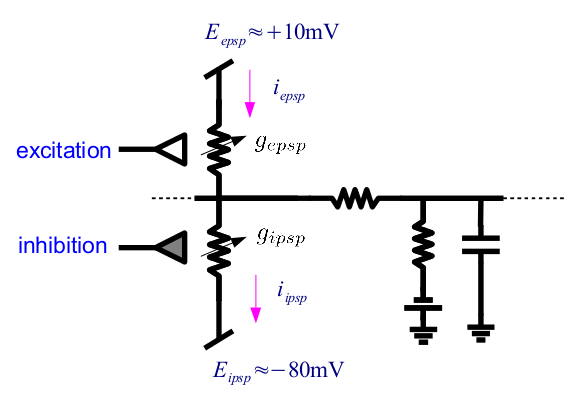
\includegraphics[width=\textwidth]{ex-inhib-elec-membrane.png}
	\end{subfigure}%
	~
	\begin{subfigure}[b]{0.5\textwidth}
		\centering
		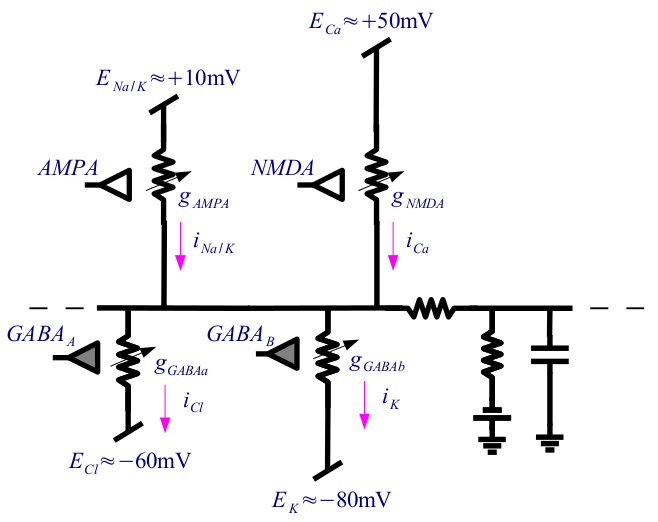
\includegraphics[width=\textwidth]{AMPA-NMDA-GABA-elec-membrane.png}
	\end{subfigure}
\end{figure}

\begin{figure}[H]
	\centering
 	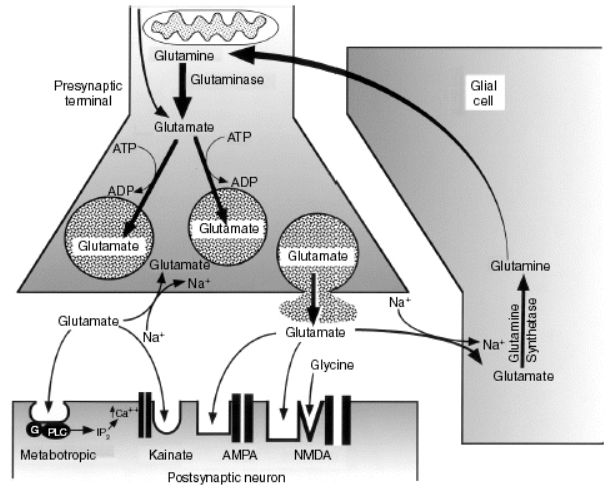
\includegraphics[scale=0.5]{glutamate-neuron.png}
\end{figure} 

\subsubsection{Glutamate receptors}
\begin{itemize}[noitemsep,nolistsep]
	\item Glutamate enables both synapses, but NMDA is voltage dependent, while AMPA is not.
	\item The receptors end up being conductive for $Na^+$ and $K^+$, as well as $Ca^{2+}$. 10 times more for $Ca^{2+}$ than the others.
	\item $E_S = 0\,mV$
	\item $Ca^{2+}$ inflow causes a calcium cascade: Phosphorylation ($PO_4$) of the channel proteines opens channels even more.
\end{itemize}

\paragraph{NMDA}
\begin{itemize}[noitemsep,nolistsep]
	\item Voltage dependent.
	\item The channel is blocked by $Mg^+$ below voltages of $-40\,mV$.
	\item The block gets pushed out with more positive voltage.
\end{itemize}

\paragraph{AMPA}
\begin{itemize}[noitemsep,nolistsep]
	\item Voltage independent.
\end{itemize}

\subsubsection{GABA}
\begin{itemize}[noitemsep,nolistsep]
	\item GABA-A is for $Cl^-$, ionotropic (fast), $-65\,mV$
	\item GABA-B is for $K^+$, metabotropic (slow), $-90\,mV$
\end{itemize}

\subsubsection{Neuromodulators}
\begin{itemize}[noitemsep,nolistsep]
	\item Neurotransmitter that is not reabsorbed by the pre-synaptic neuron or broken down into a metabolite.
	\item These end up a longer time in the cerebrospinal fluid, modulating the activity of several other neurons in the brain.
	\item For example norepinephrine, dopamine, serotonine.
\end{itemize}

\subsection{Electrical transmission}
Electrical synapses are built for speed. Electrical coupling is a way to synchronize neurons with one another (for instance, in heart muscles). In electrical synapses, the postsynaptic neuron starts to change its membrane potential almost instantaneously with the presynaptic neuron.

Rod photoreceptors are connected by electrical synapses.

\begin{itemize}
\item simple primitive system, keep firing without refractoring period
\item often symmetrical, bidirectional
\item dendrite gap junctions (connexins)
\item very fast, no synaptic delays
\item $Ca^{2+}$ independent
\item temperature insensitive
\item large synapse
\item no amplification of the signal
\item limited functions, usually excitatory
\item synchronized activity
\end{itemize}

\end{document}
